\chapter{Tabelle complete}
\label{app:tabelle}

Il \cref{cap:risultati} riporta gli aggregati; qui sono raccolti i valori per
singola run e le tabelle di supporto.

\section{Risultati per seed}

\begin{longtable}{@{}r r r r r r@{}}
\caption{Esperimento 01: risultati completi per seed. I delta sono definiti
come quantistico meno classico.}\label{tab:seed-01}\\
\toprule
\textbf{Seed} & $\mathcal{L}_c$ & $\mathcal{L}_q$ & $\Delta\mathcal{L}$ & $\PPL_c$ & $\PPL_q$ \\
\midrule
\endfirsthead
\toprule
\textbf{Seed} & $\mathcal{L}_c$ & $\mathcal{L}_q$ & $\Delta\mathcal{L}$ & $\PPL_c$ & $\PPL_q$ \\
\midrule
\endhead
42    & 2,5370 & 2,5385 & +0,0015 & 12,6411 & 12,6612 \\
137   & 2,5708 & 2,5736 & +0,0028 & 13,0764 & 13,1134 \\
256   & 2,5570 & 2,5411 & -0,0159 & 12,8971 & 12,6942 \\
512   & 2,5671 & 2,5908 & +0,0237 & 13,0282 & 13,3401 \\
1024  & 2,5251 & 2,5637 & +0,0386 & 12,4917 & 12,9832 \\
2048  & 2,5758 & 2,5665 & -0,0093 & 13,1423 & 13,0196 \\
4096  & 2,5697 & 2,5894 & +0,0197 & 13,0615 & 13,3219 \\
8192  & 2,5184 & 2,5401 & +0,0217 & 12,4084 & 12,6812 \\
16384 & 2,6341 & 2,5971 & -0,0370 & 13,9303 & 13,4245 \\
32768 & 2,5464 & 2,5549 & +0,0085 & 12,7612 & 12,8700 \\
\bottomrule
\end{longtable}

I valori degli esperimenti 02--04 sono negli aggregati descritti
nell'appendice~\ref{app:inventario}.

\section{Robustezza al rumore}

Lo sweep di rumore non fa parte della run primaria dell'esperimento 03.

\section{Tracce diagnostiche per epoca}

L'aggregato dell'esperimento 03 contiene le tracce per epoca delle 45 run; la
\cref{tab:diagnostica-03} ne riporta le medie.

\section{Parametri e tempi}

\begin{table}[htbp]
\centering
\caption[Parametri per componente]{%
Conteggio dei parametri per componente, da \file{params.json}. Il conteggio
quantistico si scompone in adapter o compressione più pesi del circuito.}
\label{tab:parametri-completi}
\small
\begin{tabular}{@{}l l r r r r@{}}
\toprule
\textbf{Esp.} & \textbf{Variante} & \textbf{Compressione} & \textbf{Circuito / MLP} & \textbf{Corpo} & \textbf{Totale} \\
\midrule
03 & \code{vanilla}      & \num{1480} & --- & \num{2759} & \num{4439} \\
03 & \code{bounded\_mlp} & \num{1480} & 400 & \num{2759} & \num{4839} \\
03 & \code{quantum\_reg} & \num{1480} & 60  & \num{2759} & \num{4499} \\
\midrule
02 & Classica    & \num{1184} & ---  & \num{1985} & \num{3169} \\
02 & Quantistica & \num{1184} & 48   & \num{1985} & \num{3217} \\
\midrule
01 & Classica    & 384 & --- & 2561 & 2945 \\
01 & Quantistica & 432 & 288 & 2561 & 3281 \\
\bottomrule
\end{tabular}
\end{table}

\begin{table}[htbp]
\centering
\caption[Tempi di esecuzione]{%
Tempi di esecuzione dell'esperimento~01, media sui seed. Device: CPU; backend
PennyLane: \code{default.qubit}. I valori misurano il costo di
\emph{simulare} il circuito e non predicono il costo su hardware quantistico
(\cref{sec:costo}).}
\label{tab:tempi}
\small
\begin{tabular}{@{}l l r r r c@{}}
\toprule
\textbf{Esp.} & \textbf{Variante} & \textbf{Totale (s)} & \textbf{Per epoca (s)} & \textbf{Valutaz.\ (s)} & \textbf{Rapporto} \\
\midrule
01 & Classica & 13,302 & 0,00887 per iter. & --- & $1{,}00\times$ \\
01 & Quantistica & 618,461 & 0,41231 per iter. & --- & $46{,}49\times$ \\
\bottomrule
\end{tabular}
\end{table}

\section{Validazione SVC dell'esperimento 04}

\begin{table}[htbp]
\centering
\caption[Esperimento 04: validazione SVC fuori campione]{%
SVC con kernel precomputato sul test ufficiale BreastMNIST. Il parametro $C$ è
selezionato con cross-validation a cinque fold sui soli dati di training.
Media $\pm$ deviazione standard su 20 sottocampioni di training.}
\label{tab:validazione-svc-04}
\small
\begin{tabular}{@{}l l c c c@{}}
\toprule
\textbf{Training 0/1} & \textbf{Kernel} & \textbf{Balanced acc.} & \textbf{AUC} & \textbf{macro-F1} \\
\midrule
\multirow{3}{*}{80/20}
 & Coseno & $0{,}5939 \pm 0{,}0919$ & $0{,}7242 \pm 0{,}0564$ & $0{,}4450 \pm 0{,}2213$ \\
 & RBF    & $0{,}5828 \pm 0{,}0871$ & $0{,}7235 \pm 0{,}0393$ & $0{,}4136 \pm 0{,}2085$ \\
 & IQP    & $0{,}5106 \pm 0{,}0204$ & $0{,}6856 \pm 0{,}0568$ & $0{,}2530 \pm 0{,}0494$ \\
\midrule
\multirow{3}{*}{50/50}
 & Coseno & $0{,}6734 \pm 0{,}0429$ & $0{,}7380 \pm 0{,}0449$ & $0{,}6409 \pm 0{,}0560$ \\
 & RBF    & $0{,}6743 \pm 0{,}0456$ & $0{,}7310 \pm 0{,}0480$ & $0{,}6427 \pm 0{,}0518$ \\
 & IQP    & $0{,}6065 \pm 0{,}0388$ & $0{,}6585 \pm 0{,}0530$ & $0{,}5674 \pm 0{,}0489$ \\
\midrule
\multirow{3}{*}{27/73}
 & Coseno & $0{,}6883 \pm 0{,}0327$ & $0{,}7454 \pm 0{,}0339$ & $0{,}6631 \pm 0{,}0385$ \\
 & RBF    & $0{,}6563 \pm 0{,}0350$ & $0{,}7213 \pm 0{,}0403$ & $0{,}6318 \pm 0{,}0472$ \\
 & IQP    & $0{,}5688 \pm 0{,}0419$ & $0{,}6632 \pm 0{,}0635$ & $0{,}5558 \pm 0{,}0512$ \\
\bottomrule
\end{tabular}
\end{table}

\section{Figure di supporto}

\begin{figure}[htbp]
\centering
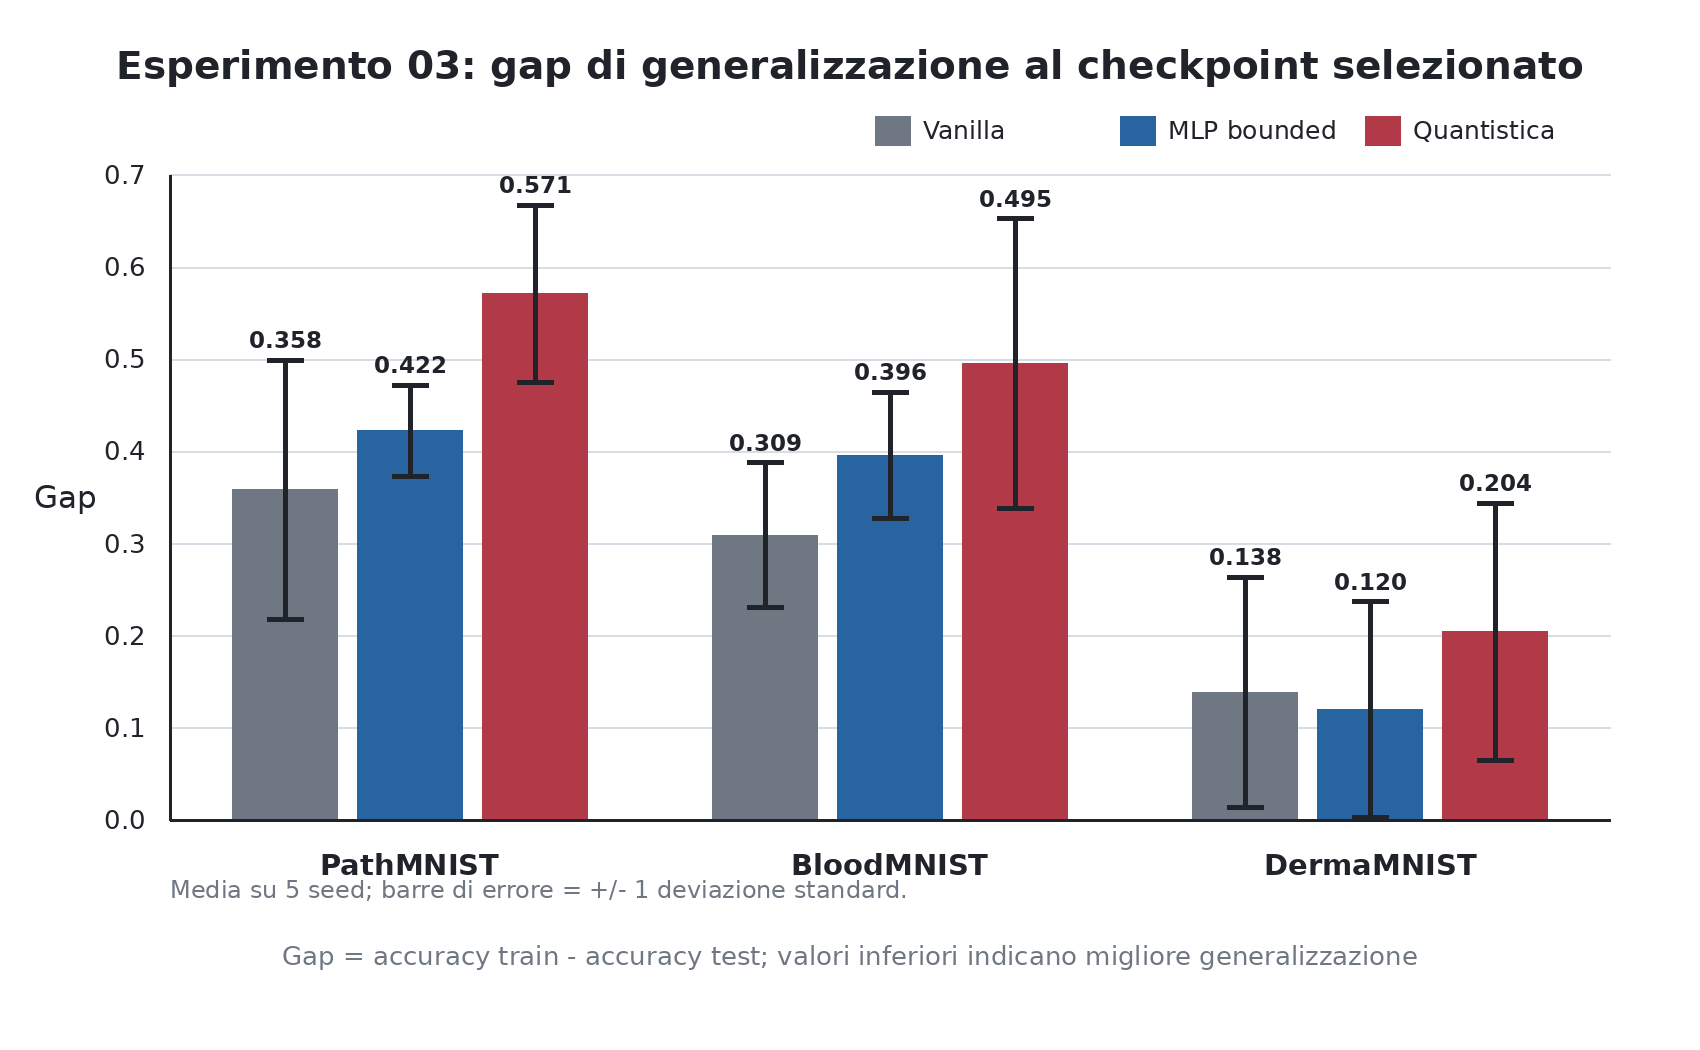
\includegraphics[width=.72\textwidth]{figure/experiment_03_gap_by_dataset.png}
\caption[Esperimento 03: gap per dataset]{Gap medio di generalizzazione nelle
tre varianti \code{vanilla}, \code{bounded\_mlp} e \code{quantum\_reg} (in figura
«Vanilla», «MLP bounded» e «Quantistica»); barre: una deviazione standard sui
seed.}
\label{fig:gap-03}
\end{figure}

\begin{figure}[htbp]
  \centering
  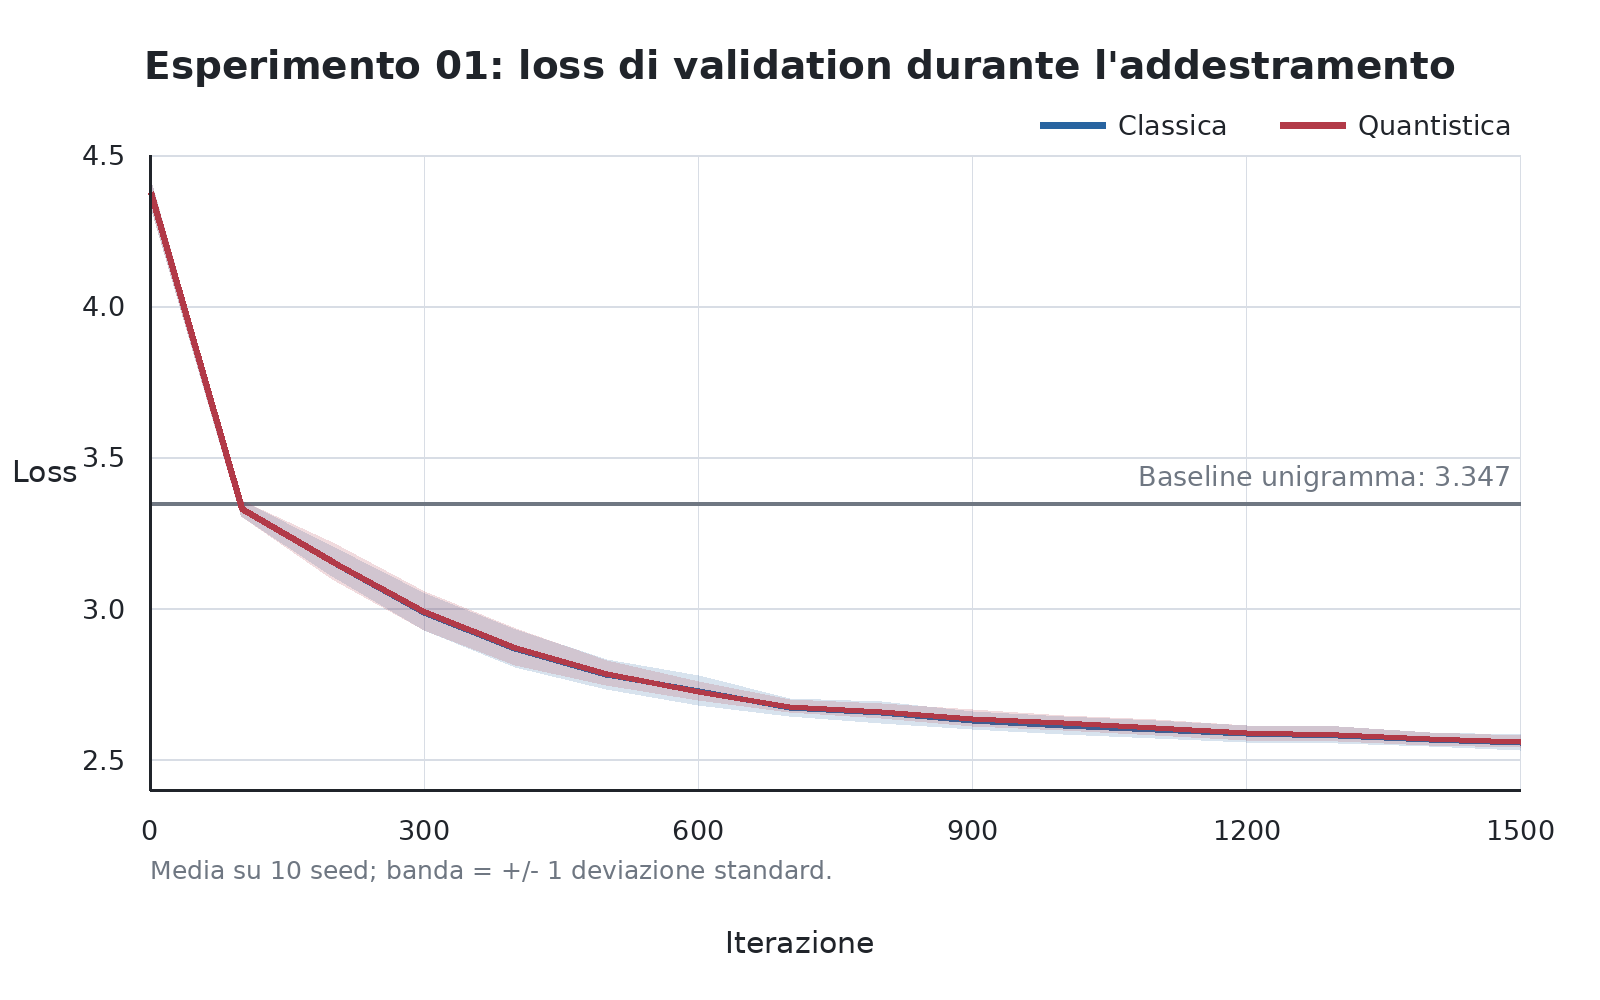
\includegraphics[width=.72\textwidth]{figure/experiment_01_learning_curves.png}
  \caption[Esperimento 01: curve di validation]{Loss di validation media sui
  dieci seed; la banda rappresenta una deviazione standard. La linea orizzontale
  è la baseline unigramma sullo split di validation. Le curve delle due varianti
  sono praticamente sovrapposte; il confronto quantitativo è nella
  \cref{fig:paired-01}.}
  \label{fig:curve-01}
\end{figure}

\begin{figure}[htbp]
\centering
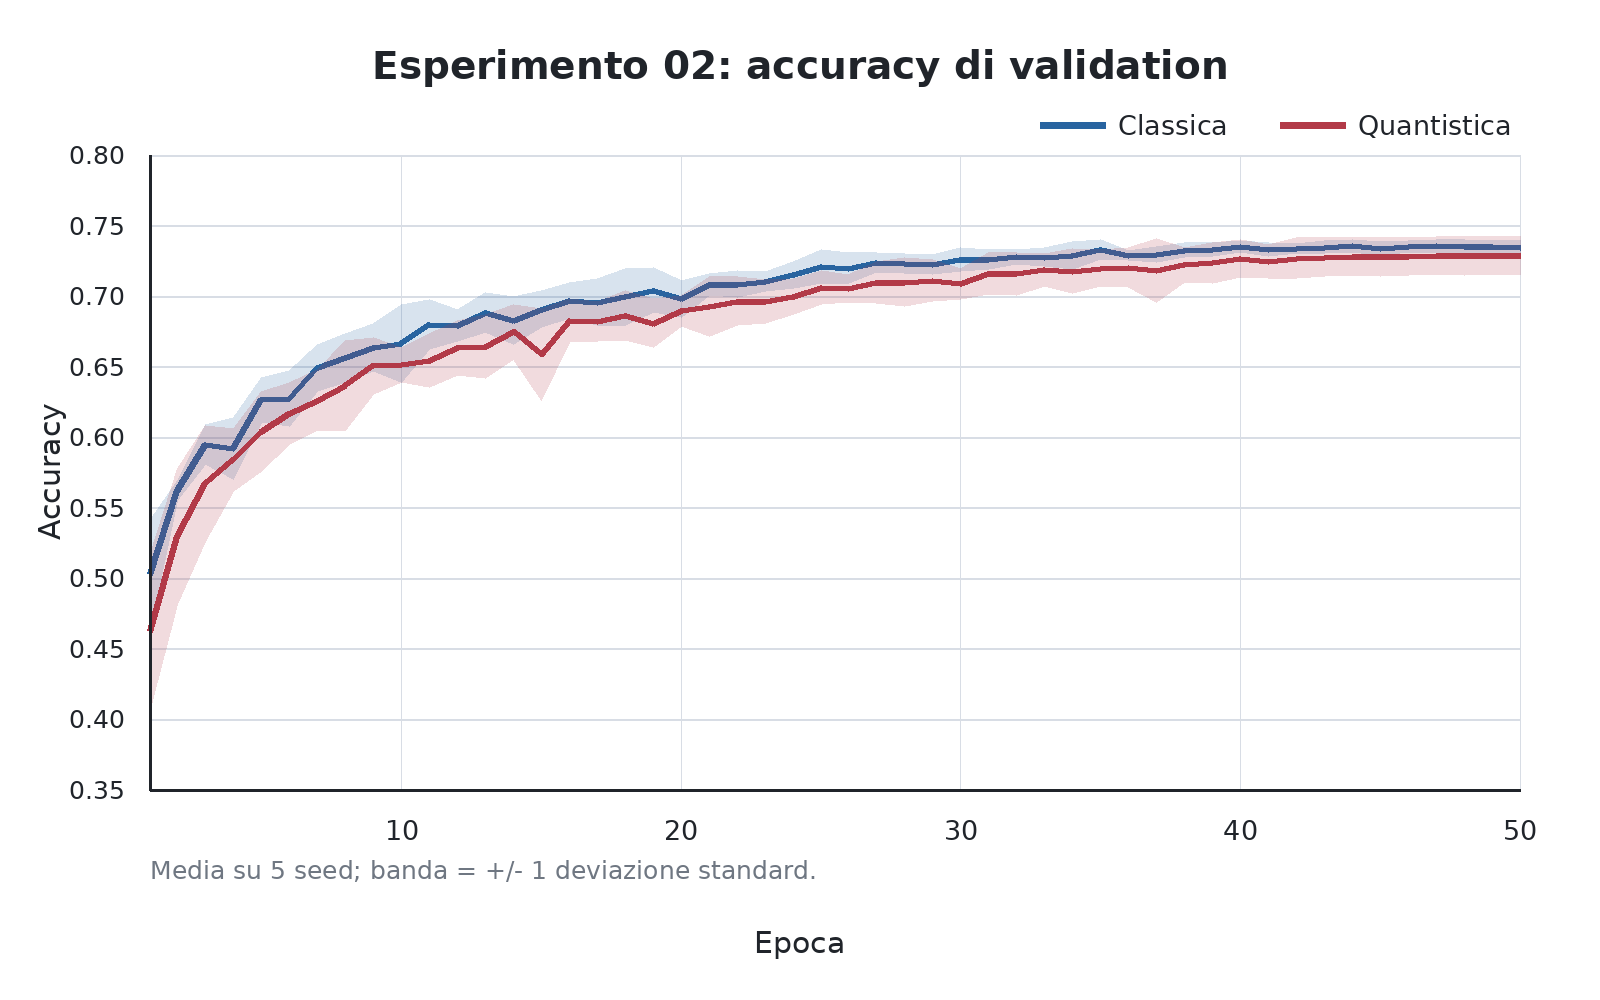
\includegraphics[width=.72\textwidth]{figure/experiment_02_learning_curves.png}
\caption[Esperimento 02: curve di validation]{Accuracy di validation media sui
cinque seed per le varianti classica e quantistica; la banda rappresenta una
deviazione standard.}
\label{fig:curve-02}
\end{figure}
